\paragraph{QuizziPedia::Front-End::Services::SearchService}
\begin{figure}[ht]
	\centering
	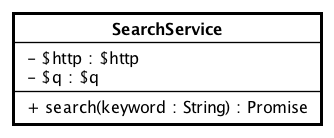
\includegraphics[scale=0.80]{UML/Classi/Front-End/QuizziPedia_Front-end_Services_SearchService.png}
	\caption{QuizziPedia::Front-End::Services::SearchService}
\end{figure}\FloatBarrier
\begin{itemize}
	\item \textbf{Descrizione}: questa classe permette di gestire il recupero dei dati dal back-end a seguito di una ricerca effettuata da un utente;
	\item \textbf{Utilizzo}: fornisce le funzionalità per recuperare dal back-end delle informazioni basandosi sulle \textit{keyword\ped{G}} inserite dall'utente;
	\item \textbf{Relazione con altre classi:}
	\begin{itemize}
		\item \textit{OUT} \texttt{SearchController}: questa classe permette di gestire la ricerca di questionari e utenti all'interno dell'applicazione.
	\end{itemize}
	\item \textbf{Attributi:}
	\begin{itemize}
		\item \texttt{-} \texttt{\$http: \$http} \\ Campo dati che contiene un riferimento al servizio \$http che permette la comunicazione con il protocollo \textit{HTTP\ped{G}};
		\item \texttt{-} \texttt{\$q: \$q} \\ Campo dati che contiene un riferimento a \$q, un servizio offerto da \textit{AngularJS\ped{G}} per la gestione, tramite \textit{Promise\ped{G}}, di chiamate asincrone. 
	\end{itemize}
	\item \textbf{Metodi:}
	\begin{itemize}
		\item \texttt{+} \texttt{SearchService(\$http: \$http, \$q: \$q)} \\ Metodo costruttore della classe. \\
		\textbf{Parametri}:
		\begin{itemize}
			\item \texttt{\$http: \$http} \\ Campo dati contenente un riferimento al servizio \$http creato da \textit{AngularJS\ped{G}} per facilitare la comunicazione mediante protocollo \textit{HTTP\ped{G}};
			\item \texttt{\$q: \$q} \\ Campo dati contenente un riferimento al servizio \$q creato da \textit{AngularJS\ped{G}} per facilitare la gestione di funzione asincrone mediante l’utilizzo delle \textit{Promise\ped{G}};
		\end{itemize}
		\item \texttt{+} \texttt{searchUsers(keyword: String): Promise} \\Metodo che serve per recuperare la lista di utenti dopo una ricerca. Il metodo ritorna una \textit{Promise\ped{G}}. In caso la \textit{Promise\ped{G}} venga rifiutata, verrà restituito al \texttt{SearchController} un oggetto \texttt{ErrorModelInfo} contenente tutti i dettagli dell'errore. In caso la \textit{Promise\ped{G}} venga accettata, verrà restituito al chiamante del metodo il risultato della chiamata.\\
		\textbf{Parametri}:
		\begin{itemize}
			\item \texttt{keyword: String} \\ Parametro che rappresenta la parola da cercare.
		\end{itemize}
		\item \texttt{+} \texttt{searchQuestionnaire(keyword: String): Promise} \\Metodo che serve per recuperare la lista dei questionari dopo una ricerca. Il metodo ritorna una \textit{Promise\ped{G}}. In caso la \textit{Promise\ped{G}} venga rifiutata, verrà restituito al \texttt{SearchController} un oggetto \texttt{ErrorModelInfo} contenente tutti i dettagli dell'errore. In caso la \textit{Promise\ped{G}} venga accettata, verrà restituito al chiamante del metodo il risultato della chiamata.\\
		\textbf{Parametri}:
		\begin{itemize}
			\item \texttt{keyword: String} \\ Parametro che rappresenta la parola da cercare.
		\end{itemize}
	\end{itemize}
\end{itemize}